\chapter{Report on present investigations:}
\section{Raspberry Pi3}{
	\begin{figure}[H]
		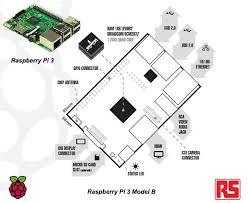
\includegraphics[width=0.9\textwidth]{images.jpg} % first figure itself
		\caption{Raspberry Pi 3}
		\label{trans}
	\end{figure}
	The Raspberry Pi 3 is the third generation Raspberry Pi. This powerful
    credit-card sized single board computer can be used for many applications
    and supersedes the Raspberry Pi 2 Model. Whilst maintaining the popular board format the Raspberry Pi 3 Model
    B brings you a more powerful processer, 10x faster than the first generation
    Raspberry Pi. Additionally it adds wireless LAN & Bluetooth connectivity
    making it the ideal solution for powerful connected designs. It has a HDMI (rev 1.3 & 1.4 Composite RCA (PAL and NTSC).It uses Broadcom BCM2387 chipset with a
    1.2GHz Quad-Core ARM Cortex-A53 and 802.11 b/g/n Wireless LAN and Bluetooth 4.1 (Bluetooth Classic and LE). It also has a 1GB LPDDR2 memory. Operating System Boots from Micro SD card, running a version of the Linux operating system or
    Windows 10 IoT.
	%\begin{equation}
	%	C = 0.7 \times I /(\Delta V \times F)
	%\end{equation}
	
}
\section{ACS712 Module Current Sensor}{
	%\subsection{Calculate the Maximum Switch Current}
	\begin{figure}[H]
	    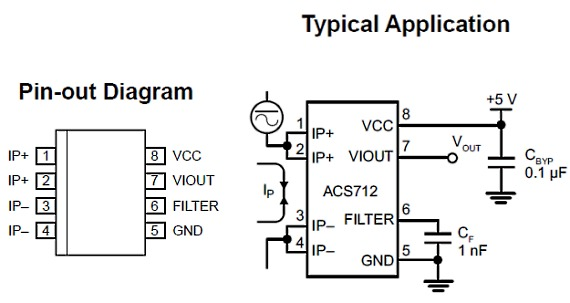
\includegraphics[width=0.9\textwidth]{PinDiagrams.jpg}
	    \caption{ACS712}
	    \label{fig:my_label}
	\end{figure}
	The Allegro™ ACS712 provides economical and precise solutions for AC or DC current sensing in industrial, commercial, and communications systems.The device consists of a precise, low-offset, linear Hall circuit with a copper conduction path located near the surface of the die. Applied current flowing through this copper conduction path generates a magnetic field which the Hall IC converts into a proportional voltage. Device accuracy is optimized through the close proximity of the magnetic signal to the Hall transducer. A precise, proportional voltage is provided by the low-offset, chopper-stabilized BiCMOS Hall IC, which is programmed for accuracy after packaging. The internal resistance of this conductive path is 1.2 mΩ typical, providing low power loss. The thickness of the copper conductor allows survival of the device at up to 5× overcurrent conditions. The terminals of the conductive path are electrically isolated from the signal leads (pins 5 through 8). This allows the ACS712 to be used in applications requiring electrical isolation without the use of opto-isolators or other costly isolation techniques. It requires a 4.5-5.5V power supply. It takes input current of 0-30A and produces output voltage of 2.5-5V.
%	\begin{equation}\label{eq1}
%	D = \frac{V_{out}}{V_{IN(max)} \times \eta}
%	\end{equation}
%	Where,\\
%	$V_{IN(max)}$ = maximum input voltage\\
%	\subsection{Inductor Selection}
%	\begin{equation}
%	L= \frac{Vout \times (Vin-Vout)}{ \Delta I_L \times fs\times vin} 
%	\end{equation}
%	Where,\\
%	$V_{IN}$ = typical input voltage\\
%	$V_{OUT}$ = desired output voltage\\
%	$f_S$ = minimum switching frequency of the converter\\
%	$\Delta I_L$ = estimated inductor ripple current\\
%	$\Delta I_L$ = estimated inductor ripple current\\
%	$I_{OUT(max)}$ = maximum output current necessary in the application\\
	
%	\subsection{Rectifier Diode Selection}
}
\section{ADS1115 Analog to Digital Converter}{
%\subsection{Power Supply Unit of the Peltier TEC1-12706}
\begin{figure}[H]
	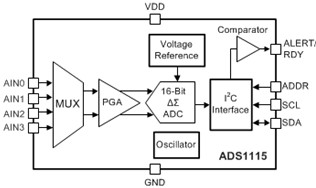
\includegraphics[width=0.9\textwidth]{fbd_sbas444c.jpg} % first figure itself
	\caption{ADC circuit}
	\label{ADC}
\end{figure}
The ADS1115 device is a precision, low-power, 16-bit, I2C-compatible, analog-to-digital converters (ADCs) offered in an ultra-small, leadless, X2QFN-10 package, and a VSSOP-10 package. The ADS111x devices incorporate a low-drift voltage reference and an oscillator. The ADS1114 and ADS1115 also incorporate a programmable gain amplifier (PGA) and a digital comparator. These features, along with a wide operating supply range, make the ADS111x well suited for power- and space-constrained, sensor measurement applications.

The ADS1115 perform conversions at data rates up to 860 samples per second (SPS). The PGA offers input ranges from ±256 mV to ±6.144 V, allowing precise large- and small-signal measurements. The ADS1115 features an input multiplexer (MUX) that allows two differential or four single-ended input measurements. Use the digital comparator for under- and overvoltage detection.

The ADS111x operate in either continuous-conversion mode or single-shot mode. The devices are automatically powered down after one conversion in single-shot mode; therefore, power consumption is significantly reduced during idle periods. It has a resolution of 16 bits, sample rate of 860SPS, 4 Input channel, I2C, Interface, 2-5.5V Power Supply,

}
\section{User Interface}
{The user interface uses a Python Micro-Framework called Flask which is used to build web applications. The Flask framework encodes the real time Python Variables into a JavaScript Object Notation(JSON) string. The JSON string is then read into the HTML file using Asynchronous JavaScript And XML(AJAX) requests. These requests are periodically refreshed using the Auto-Refresh function in AJAX.}
\begin{figure}[H]
	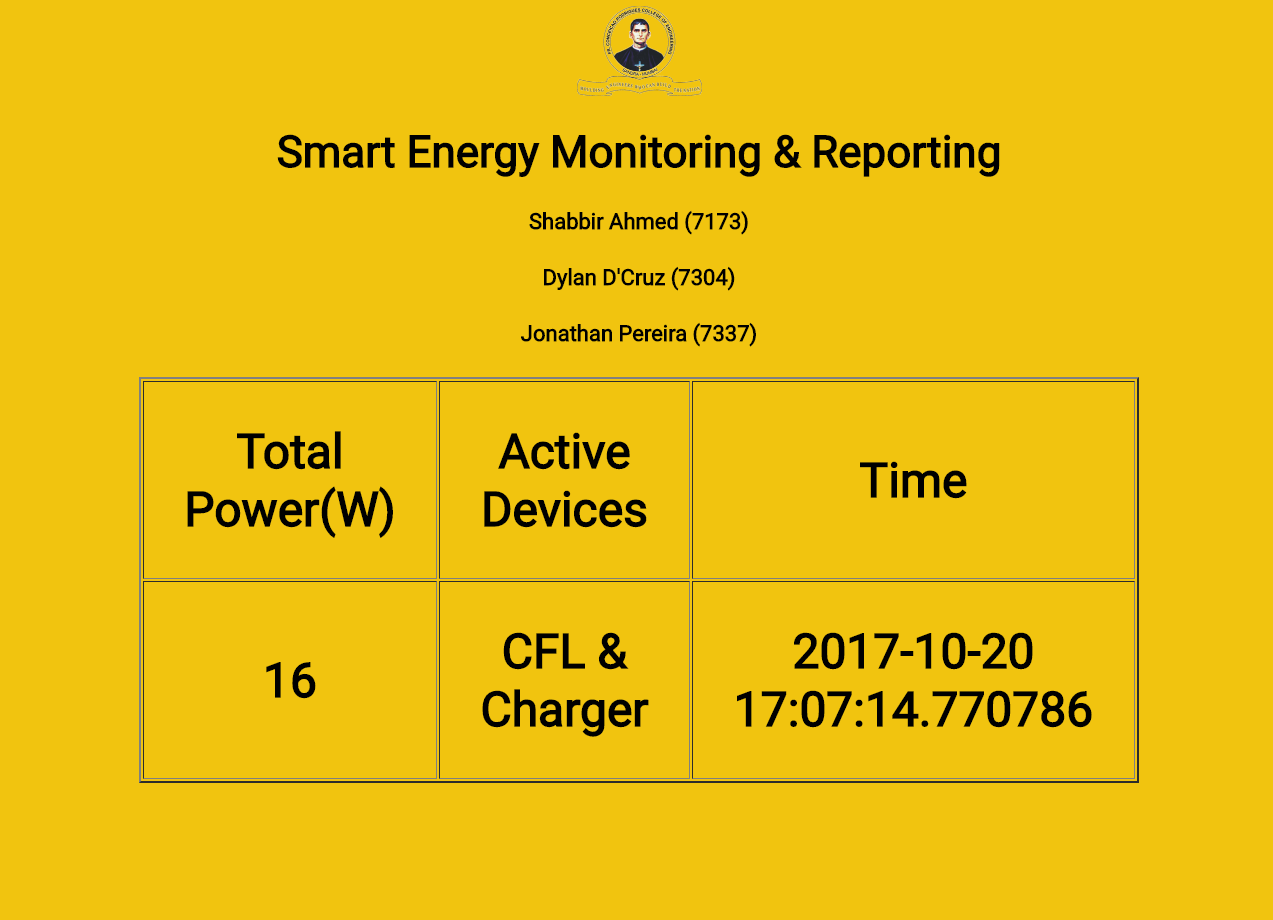
\includegraphics[width=0.9\textwidth]{Demo1.PNG} % first figure itself
	\caption{HTML-Based UI}
	\label{UI}
\end{figure}
{The user interface displays various system parameters such as Total Power being Consumed, Active Devices and the Real Time Clock. Additional parameters such as Estimated Monthly Electricity bill can be added in the future.}

\section{Classification Algorithm (KNN)}{
In machine learning and statistics, classification is the problem of identifying to which of a set of categories (sub-populations) a new observation belongs, on the basis of a training set of data containing observations (or instances) whose category membership is known. An example would be assigning a given email into "spam" or "non-spam" classes or assigning a diagnosis to a given patient as described by observed characteristics of the patient (gender, blood pressure, presence or absence of certain symptoms, etc.). Classification is an example of pattern recognition.

In the terminology of machine learning, classification is considered an instance of supervised learning, i.e. learning where a training set of correctly identified observations is available. The corresponding unsupervised procedure is known as clustering, and involves grouping data into categories based on some measure of inherent similarity or distance.

Often, the individual observations are analyzed into a set of quantifiable properties, known variously as explanatory variables or features. These properties may variously be categorical (e.g. "A", "B", "AB" or "O", for blood type), ordinal (e.g. "large", "medium" or "small"), integer-valued (e.g. the number of occurrences of a particular word in an email) or real-valued (e.g. a measurement of blood pressure). Other classifiers work by comparing observations to previous observations by means of a similarity or distance function.

An algorithm that implements classification, especially in a concrete implementation, is known as a classifier. The term "classifier" sometimes also refers to the mathematical function, implemented by a classification algorithm, that maps input data to a category.
 
KNN ( k Nearest Neighbours)
In pattern recognition, the k-nearest neighbors algorithm (k-NN) is a non-parametric method used for classification and regression. In both cases, the input consists of the k closest training examples in the feature space. The output depends on whether k-NN is used for classification or regression:

In k-NN classification, the output is a class membership. An object is classified by a majority vote of its neighbors, with the object being assigned to the class most common among its k nearest neighbors (k is a positive integer, typically small). If k = 1, then the object is simply assigned to the class of that single nearest neighbor.
In k-NN regression, the output is the property value for the object. This value is the average of the values of its k nearest neighbors.
k-NN is a type of instance-based learning, or lazy learning, where the function is only approximated locally and all computation is deferred until classification. The k-NN algorithm is among the simplest of all machine learning algorithms.

Both for classification and regression, it can be useful to assign weight to the contributions of the neighbors, so that the nearer neighbors contribute more to the average than the more distant ones. For example, a common weighting scheme consists in giving each neighbor a weight of 1/d, where d is the distance to the neighbor.

The neighbors are taken from a set of objects for which the class (for k-NN classification) or the object property value (for k-NN regression) is known. This can be thought of as the training set for the algorithm, though no explicit training step is required.

A peculiarity of the k-NN algorithm is that it is sensitive to the local structure of the data.[citation needed] The algorithm is not to be confused with k-means, another popular machine learning technique. 
 Following example would help us to understand better :
 The test sample (green circle) should be classified either to the first class of blue squares or to the second class of red triangles. If k = 3 (solid line circle) it is assigned to the second class because there are 2 triangles and only 1 square inside the inner circle. If k = 5 (dashed line circle) it is assigned to the first class (3 squares vs. 2 triangles inside the outer circle). 
\begin{figure}
    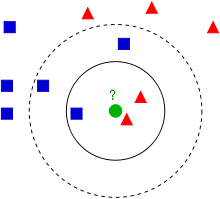
\includegraphics[width=0.9\textwidth]{Knn.png}
    \caption{K Nearest Neighbour}
    \label{fig:my_label}
\end{figure}
}